% Provenance (never printed): see sources/outline_sources.md (Year 2: humidity variables;
% Clausius--Clapeyron applied; dry and moist adiabats; thermodynamic diagrams; convective
% instability; cloud microphysics). Definitions after the NWS glossary; skew-T lines, CAPE classes
% and the lifted index after the NWS Houston/Galveston training page; saturation data from the
% NIST WebBook (IAPWS-95) and IAPWS R14-08; the empirical formula as used by Su and others
% (2026); kappa-Koehler theory after Petters and Kreidenweis (2007); CCN numbers after Andreae
% (2009); the processes of microphysics after Morrison and others (2020). The sounding is the
% real 12 UTC sounding of Norman, Oklahoma, 16 April 2026 (IGRA2); every curve and number from
% figdata/bachelor-2/thermo.py; exercise and problem values in the Book 4 scratch calculator
% calc/ch21.py.
\chapter{大气热力学}\label{ch:b2:atmospheric-thermodynamics}

2026 年 4 月 16 日 12 UTC，一只探空气球从俄克拉荷马州诺曼的气象站升空，
如同每天此时从八百多个站点放飞的气球一样。它所携带的仪器
通过无线电回传一条竖直廓线，预报员一眼即可读懂：近地面空气
几近饱和，600 米高处有一层薄薄的暖盖，其上气温
随高度迅速下降，延续约 10 千米。若将近地面空气抬升穿过暖盖，它将发现自己
在对流层的大部分高度上比周围空气更暖，每千克约有
2000 焦耳可供上升消耗。本章学习由探空曲线读取这一能量：空气能容纳多少
水汽，上升气块在凝结前后如何降温，气象学家的图解如何把面积
换算为能量，以及云滴究竟如何形成。
% ledger: data:b4-sounding, nws4:upperair, nws4:cape

\begin{recall}
\textbf{来自物理学教材}：饱和\omterm{def:b2:atmospheric-thermodynamics:moist-air}{水汽压}、相对湿度、露点，
潜热、克劳修斯–克拉珀龙关系及其积分形式；成核和
过冷；热力学第一定律、绝热过程和理想气体的热容。
\textbf{来自化学教材}：分压、拉乌尔定律、表面张力以及开尔文
方程。\textbf{来自中学各分册}：\omterm{def:b2:atmospheric-thermodynamics:lcl}{凝结高度}及其
每度 \qty{125}{m} 的规则、稳定与不稳定空气、\omterm{def:b2:atmospheric-thermodynamics:microphysics}{凝结核}、暖雨与
冰晶过程。\textbf{来自本科一年级分册}：标准大气、环境
递减率与干绝热递减率（$\Gamma_d = \qty{9.8}{K/km}$）、气块、位
温、静力稳定度、逆温以及气压高度方程。
\end{recall}

全章约定：干空气的 $R_d = R/M_d = \qty{287.0}{J.kg^{-1}.K^{-1}}$，其摩尔质量
为 \qty{28.97}{g/mol}；水汽的 $R_v = R/M_w = \qty{461.5}{J.kg^{-1}.K^{-1}}$，其摩尔
质量为 \qty{18.0153}{g/mol}；$\varepsilon = M_w/M_d = 0.622$；$c_p = \tfrac72 R_d =
\qty{1004.5}{J.kg^{-1}.K^{-1}}$（本科一年级分册，热容比为 1.4）；
$g = \qty{9.81}{m.s^{-2}}$；以及三相点处的
汽化潜热 $L = \qty{2.501e6}{J/kg}$。
% ledger: const:R, earth:Mmol, nist4:water-mw, nasa:grc-gamma, const:gn, nist4:water-sat

\section{湿空气}\label{sec:b2:atmospheric-thermodynamics:moist-air}

空气是干空气与水汽的混合物，两者都近似为理想气体。物理学教材
用相对湿度和露点来度量其含水量；而上升的气块需要在膨胀时
仍保持不变的度量。

\begin{definition}[水汽压；混合比；比湿]\label{def:b2:atmospheric-thermodynamics:moist-air}
湿空气的\emph{水汽压}\index{水汽压} $e$ 为其中水汽的
分压。其\emph{混合比}\index{混合比}为 $r = m_v/m_d$，即
同一体积中单位质量干空气所含的水汽质量，而其
\emph{比湿}\index{比湿}为 $q = m_v/(m_d + m_v)$，即单位质量湿空气中的水汽质量。
二者通常以克每千克表示。
\end{definition}
% ledger: nws4:humidity

\begin{proposition}[湿度变量]\label{prop:b2:atmospheric-thermodynamics:humidity}
设湿空气的总压为 $p$、\omterm{def:b2:atmospheric-thermodynamics:moist-air}{水汽压}为 $e$，则
\[
  r = \frac{\varepsilon e}{p - e}, \qquad q = \frac{r}{1 + r} = \frac{\varepsilon e}{p - (1 -
  \varepsilon)e} .
\]
饱和时 $e = e_s(T)$，$r = r_s(T, p)$，即饱和\omterm{def:b2:atmospheric-thermodynamics:moist-air}{混合比}。气块膨胀或被压缩
而未得失水分时，$r$ 与 $q$ 均不改变。
\end{proposition}

\begin{proof}
在同一体积 $V$、温度 $T$ 下，每种气体各自服从以其分压表示的理想气体定律，
即 $m_v = eV/(R_vT)$，$m_d = (p - e)V/(R_dT)$，于是 $r = (R_d/R_v)\,e/(p - e)$，
且 $R_d/R_v = M_w/M_d = \varepsilon$。以 $m_v$ 除以 $m_d + m_v$ 即得 $q = r/(1 + r)$。
膨胀改变 $V$、$p$ 与 $e$，但不改变两种质量。
\end{proof}

\begin{definition}[虚温]\label{def:b2:atmospheric-thermodynamics:virtual}
湿空气的\emph{虚温}\index{虚温} $T_v$ 是指：在相同压强下，
干空气要具有相同密度所需的温度：
\[
  T_v = T\,\frac{1 + r/\varepsilon}{1 + r} \approx T\,(1 + 0.61\,r) .
\]
\end{definition}
% ledger: nws4:virtual-theta-e

这一温度名副其实，证明只需一行：湿空气的密度为
$(m_d + m_v)/V = \bigl(p - e\bigr)/(R_dT) + e/(R_vT)$，代入 $e = pr/(\varepsilon + r)$，
便等于 $p/(R_dT_v)$。水汽比干空气轻，因此在相同温度与压强下，湿空气的密度
小于干空气，仿佛温度略高一些。

\begin{example}[诺曼的空气]\label{ex:b2:atmospheric-thermodynamics:norman}
地面处探空给出 $p = \qty{971.1}{hPa}$、$T = \qty{19.0}{\celsius}$，露点为
\qty{18.5}{\celsius}。\omterm{def:b2:atmospheric-thermodynamics:moist-air}{水汽压}即露点处的饱和\omterm{def:b2:atmospheric-thermodynamics:moist-air}{水汽压}，
$e = e_s(\qty{18.5}{\celsius}) = \qty{21.5}{hPa}$（下文见\cref{prop:b2:atmospheric-thermodynamics:es}
）。则 $r = 0.622 \times 21.5/(971.1 - 21.5) = \qty{14.1}{g/kg}$，$q = \qty{13.9}{g/kg}$，
且 $T_v - T = 0.61 \times 0.0141 \times \qty{292.15}{K} = \qty{2.5}{K}$：此空气与
温度高 2.5 度的干空气一样轻。
\end{example}
% ledger: data:b4-sounding

\section{饱和水汽压}\label{sec:b2:atmospheric-thermodynamics:saturation}

对于纯水的平液面，平衡\omterm{def:b2:atmospheric-thermodynamics:moist-air}{水汽压}仅取决于
温度。物理学教材推导了其定律，即克劳修斯–克拉珀龙关系，并
在潜热为常数时积分；对水汽而言 $M L/R = L/R_v$。

\begin{proposition}[饱和水汽压]\label{prop:b2:atmospheric-thermodynamics:es}
设潜热 $L$ 为常数，则水面上的饱和\omterm{def:b2:atmospheric-thermodynamics:moist-air}{水汽压}为
\[
  e_s(T) = e_t \exp\!\Bigl[\frac{L}{R_v}\Bigl(\frac{1}{T_t} - \frac{1}{T}\Bigr)\Bigr],
  \qquad e_t = \qty{6.117}{hPa}, \quad T_t = \qty{273.16}{K}, \quad \frac{L}{R_v} =
  \qty{5419}{K},
\]
其中 $(T_t, e_t)$ 为水的三相点。
\end{proposition}
% ledger: iapws4:sublimation, nist4:water-sat

\begin{corollary}[每开尔文百分之七]\label{cor:b2:atmospheric-thermodynamics:seven}
饱和\omterm{def:b2:atmospheric-thermodynamics:moist-air}{水汽压}的相对增长率为
$\mathrm{d}\ln e_s/\mathrm{d}T = L/(R_v T^2)$：在
\qty{0}{\celsius} 时每开尔文为 \qty{7.3}{\percent}，在 \qty{20}{\celsius} 时为 \qty{6.3}{\percent}，在
\qty{30}{\celsius} 时为 \qty{5.9}{\percent}。
\end{corollary}

恒定潜热是该公式唯一的缺陷：潜热由
三相点处的 \qty{2500.9}{kJ/kg} 降至 \qty{20}{\celsius} 时的 \qty{2453.5}{kJ/kg}，因此
该公式的值随温度升高而逐渐超过实测值，在 \qty{20}{\celsius} 时偏高
\qty{1.2}{\percent}，在 \qty{30}{\celsius} 时偏高 \qty{2.5}{\percent}（见下图）。经验公式
是拟合实测数据得到的，即 $e_s = \qty{6.112}{hPa} \times \exp[17.67\,t/(t + 243.5)]$，其中
$t$ 为摄氏温度，误差保持在千分之几以内；数据产品多用此式，但
命题中的形式便于求导和理解，故本章仍予保留。
% ledger: nist4:water-sat, su26:svp

在 \qty{0}{\celsius} 以下，云中的水可以以过冷液态存在，因而饱和\omterm{def:b2:atmospheric-thermodynamics:moist-air}{水汽压}有
两种：即对液态水与对冰的饱和\omterm{def:b2:atmospheric-thermodynamics:moist-air}{水汽压}。后者较低，因为升华潜热
比汽化潜热多出一个熔化潜热。相对于过冷水滴饱和的空气，
对冰则处于\omterm{def:b2:atmospheric-thermodynamics:microphysics}{过饱和}状态，\omterm{def:b2:atmospheric-thermodynamics:microphysics}{过饱和}度在
\qty{-10}{\celsius} 时为 \qty{10}{\percent}，在 \qty{-20}{\celsius} 时为 \qty{22}{\percent}。末节将回到
这一差异。
% ledger: iapws4:sublimation, su26:svp

\begin{omfigure}
\centering
% figdata/bachelor-2/thermo.py parts es, nist
\begin{tikzpicture}
\begin{groupplot}[group style={group size=2 by 1, horizontal sep=1.9cm},
  width=0.44\linewidth, height=5.4cm, tick label style={font=\scriptsize},
  label style={font=\small}]
\nextgroupplot[xmin=-40, xmax=40, ymin=0, ymax=80, xlabel={温度 (\unit{\celsius})},
  ylabel={饱和水汽压 (\unit{hPa})}, legend pos=north west,
  legend style={font=\scriptsize, draw=none, fill=none}, legend cell align=left]
\addplot[ocBlue, thick] table[x=T_C, y=cc] {figdata/out/bachelor-2-thermo-es.dat};
\addlegendentry{命题}
\addplot[black, densely dashed] table[x=T_C, y=emp] {figdata/out/bachelor-2-thermo-es.dat};
\addlegendentry{经验公式}
\addplot[only marks, mark=*, mark size=1.4pt, ocRed] table[x=T_C, y=es_hPa]
  {figdata/out/bachelor-2-thermo-nist.dat};
\addlegendentry{实测 (IAPWS-95)}
\nextgroupplot[xmin=-40, xmax=0, ymin=1, ymax=1.5, xlabel={温度 (\unit{\celsius})},
  ylabel={$e_s(\text{水})/e_s(\text{冰})$}]
\addplot[omMeth, thick, unbounded coords=discard] table[x=T_C, y=wi]
  {figdata/out/bachelor-2-thermo-es.dat};
\draw[black!40, densely dotted] (axis cs:-10,1) -- (axis cs:-10,1.1035) -- (axis cs:-40,1.1035);
\node[font=\scriptsize, anchor=south west] at (axis cs:-10,1.1035) {1.10};
\draw[black!40, densely dotted] (axis cs:-20,1) -- (axis cs:-20,1.218) -- (axis cs:-40,1.218);
\node[font=\scriptsize, anchor=south west] at (axis cs:-20,1.218) {1.22};
\end{groupplot}
\end{tikzpicture}
\par\smallskip{\small 左：水面饱和\omterm{def:b2:atmospheric-thermodynamics:moist-air}{水汽压}，由
\cref{prop:b2:atmospheric-thermodynamics:es}、经验公式及实测值给出。右：
过冷水（经验公式）与
冰（IAPWS 升华方程）的饱和\omterm{def:b2:atmospheric-thermodynamics:moist-air}{水汽压}之比。}
\end{omfigure}
% ledger: nist4:water-sat, iapws4:sublimation, su26:svp

\section{湿空气的抬升}\label{sec:b2:atmospheric-thermodynamics:ascent}

上升而不与外界交换热量的气块，以干绝热递减率降温，并保持其
位温；若不发生凝结，则\omterm{def:b2:atmospheric-thermodynamics:moist-air}{混合比}保持不变。其\omterm{def:b2:atmospheric-thermodynamics:moist-air}{水汽压}
$e = pr/(\varepsilon + r)$ 随气压下降而减小，但其饱和\omterm{def:b2:atmospheric-thermodynamics:moist-air}{水汽压}
随温度下降得更快。两者相交于一个高度，该高度由高中分册依一条规则求得。

\begin{definition}[抬升凝结高度]\label{def:b2:atmospheric-thermodynamics:lcl}
气块的\emph{抬升凝结高度}\index{抬升凝结高度}（LCL）是指
气块被干绝热抬升时达到饱和的高度。它即
高中分册中的\emph{凝结高度}\index{凝结高度}，也就是
抬升形成的云的平坦云底高度。
\end{definition}
% ledger: nws4:lcl

\begin{proposition}[抬升凝结高度的估算]\label{prop:b2:atmospheric-thermodynamics:lcl}
温度为 $T$、露点为 $T_d$ 的气块，约在
\[
  z_{\text{LCL}} \approx \frac{T - T_d}{\Gamma_d - \Gamma_{\text{露点}}}, \qquad
  \Gamma_{\text{露点}} = \frac{g R_v T_d^2}{L R_d T} \approx \qty{1.8}{K/km},
\]
高于其出发高度，露点差每差一开尔文约为 \qty{125}{m}。
\end{proposition}

\begin{proof}
气块温度以 $\Gamma_d$ 下降。其露点是使其\omterm{def:b2:atmospheric-thermodynamics:moist-air}{水汽压}
$e$ 恰好饱和的温度；$r$ 不变时，$e$ 正比于 $p$，故
$\mathrm{d}\ln e = \mathrm{d}\ln p = -g\,\mathrm{d}z/(R_dT)$，由静力平衡得。由
\cref{prop:b2:atmospheric-thermodynamics:es}，$\mathrm{d}\ln e = L\,\mathrm{d}T_d/(R_vT_d^2)$。
因此 $\mathrm{d}T_d/\mathrm{d}z = -gR_vT_d^2/(LR_dT) = -\Gamma_{\text{露点}}$，露点同样下降，
但下降较慢。差值 $T - T_d$ 以 $\Gamma_d - \Gamma_{\text{露点}}$ 的速率缩小。取
$T \approx T_d \approx \qty{288}{K}$，$\Gamma_{\text{露点}} = \qty{1.8}{K/km}$，且 $1/(9.8 - 1.8)$
千米每开尔文，即 \qty{125}{m}。
\end{proof}

在诺曼，露点差为 \qty{0.5}{K}，地面空气将在
抬升 \qty{63}{m}、气压为 \qty{964}{hPa} 时凝结。完整计算沿干绝热线，并
采用饱和\omterm{def:b2:atmospheric-thermodynamics:moist-air}{混合比}而不作线性化，得 \qty{64}{m}。
% ledger: data:b4-sounding

在\omterm{def:b2:atmospheric-thermodynamics:lcl}{抬升凝结高度}以上，气块随上升而凝结。凝结释放潜热，气块
降温较慢。

\begin{definition}[湿绝热递减率；湿绝热线]\label{def:b2:atmospheric-thermodynamics:moist-adiabat}
称\emph{湿绝热递减率}\index{湿绝热递减率} $\Gamma_s$ 为
饱和气块随上升而降温的速率，其水汽凝结以
保持饱和。在以温度与气压为坐标的图上，它所沿的曲线是一条
\emph{湿绝热线}\index{湿绝热线}。若假定凝结水即刻落出，
则此上升过程称为假绝热。
\end{definition}
% ledger: nws4:malr

\begin{proposition}[湿绝热递减率]\label{prop:b2:atmospheric-thermodynamics:gamma-s}
对于假绝热上升，设 $r_s = r_s(T, p)$，
\[
  \Gamma_s = g\,\frac{1 + \dfrac{L r_s}{R_d T}}{c_p + \dfrac{L^2 r_s}{R_v T^2}} .
\]
它趋于 $\Gamma_d = g/c_p$，此时 $r_s$ 趋于零；其余情形下均更小。
\end{proposition}

\begin{proof}
取单位质量干空气，气块接受其所凝结水汽的潜热 $-L\,\mathrm{d}r_s$，
则热力学第一定律为 $c_p\,\mathrm{d}T - (R_dT/p)\,\mathrm{d}p = -L\,
\mathrm{d}r_s$；结合静力平衡 $(R_dT/p)\,\mathrm{d}p = -g\,\mathrm{d}z$，得
$c_p\,\mathrm{d}T + g\,\mathrm{d}z + L\,\mathrm{d}r_s = 0$。由 $r_s \approx \varepsilon e_s/p$ 可得，
$\mathrm{d}r_s = r_s\,(\mathrm{d}\ln e_s - \mathrm{d}\ln p) = r_s\bigl(L\,\mathrm{d}T/(R_vT^2) +
g\,\mathrm{d}z/(R_dT)\bigr)$。代入并合并 $\mathrm{d}T$ 与
$\mathrm{d}z$ 的项，即得 $-\mathrm{d}T/\mathrm{d}z = \Gamma_s$。
\end{proof}

递减率取决于可供凝结的水量。在 \qty{1000}{hPa} 下，各温度处的递减率依次为
\qty{6.5}{K/km}（\qty{0}{\celsius}）、\qty{5.2}{K/km}（\qty{10}{\celsius}）、\qty{4.2}{K/km}（\qty{20}{\celsius}）、
\qty{3.4}{K/km}（\qty{30}{\celsius}）；在对流层高处，
即 \qty{200}{hPa} 且 \qty{-60}{\celsius} 时，又回到 \qty{9.6}{K/km}，几乎与干绝热递减率相当。
因此\omterm{def:b2:atmospheric-thermodynamics:moist-adiabat}{湿绝热线}在温暖地面附近很陡，在高空则向干绝热线靠拢。
% ledger: nws4:malr

\begin{definition}[相当位温]\label{def:b2:atmospheric-thermodynamics:theta-e}
气块的\emph{相当位温}\index{相当位温} $\theta_e$ 是指
若将其抬升至全部水汽凝结并落出，
再沿干绝热线降至 \qty{1000}{hPa}，所具有的温度。其良好近似为
\[
  \theta_e \approx \theta \exp\!\Bigl(\frac{L r}{c_p T_{\text{LCL}}}\Bigr),
\]
其中 $\theta$ 为位温，$T_{\text{LCL}}$ 为该气块
\omterm{def:b2:atmospheric-thermodynamics:lcl}{抬升凝结高度}处的温度。
\end{definition}
% ledger: nws4:virtual-theta-e

位温仅在干绝热上升中守恒；$\theta_e$ 在此近似下
在干绝热与饱和上升中均守恒，因其所计入的已释放热量
恰等于凝结所释放的热量。它标识\omterm{def:b2:atmospheric-thermodynamics:moist-adiabat}{湿绝热线}，正如 $\theta$ 标识干绝热线。
诺曼地面空气的 $\theta = 292.15 \times (1000/971.1)^{2/7} = \qty{294.6}{K}$，
$\theta_e = 294.6 \exp[2.501 \times 10^6 \times 0.0141/(1004.5 \times 291.5)] = \qty{332}{K}$。
% ledger: data:b4-sounding

\section{热力学图解}\label{sec:b2:atmospheric-thermodynamics:diagrams}

\begin{definition}[大气探空]\label{def:b2:atmospheric-thermodynamics:sounding}
\emph{大气探空}\index{大气探空}是指对某地上空大气的
压强、温度、湿度与风的竖直剖面所作的测量，测量仪器
由高空携带，通常为气球下挂的探空仪。
\end{definition}
% ledger: nws:radiosonde, nws4:upperair

探空并非严格竖直，因为气球随风飘移；也并非
瞬时完成，因为抵达对流层高层需要数分钟；而且主要观测网
每天仅施放两次。其数据只有绘制在图上，才能
让上升气块用尺子逐段追踪，从而真正有用。
% ledger: hgx:skewt-lines

\begin{definition}[热力学图解；斜温对数压力图；温熵图]\label{def:b2:atmospheric-thermodynamics:diagram}
\emph{热力学图解}\index{热力学图解}是一种坐标为压强与温度函数的图，
图上标出等压线、等温线、干绝热线、\omterm{def:b2:atmospheric-thermodynamics:moist-adiabat}{湿绝热线}、
以及等饱和\omterm{def:b2:atmospheric-thermodynamics:moist-air}{混合比}线，并将探空绘制为
两条曲线，即温度曲线与露点曲线。在\emph{斜温对数压力图}\index{斜温对数压力图}上，
竖直坐标为 $-\ln p$，水平坐标为
$T + k\ln(p_0/p)$，使等压线为水平线，等温线向右上方倾斜。
\emph{温熵图}\index{温熵图}以温度与单位质量的
熵 $c_p\ln\theta$ 为坐标，使等温线与干绝热线成为
相互垂直的直线。
\end{definition}
% ledger: hgx:skewt-lines

\begin{proposition}[面积即能量]\label{prop:b2:atmospheric-thermodynamics:areas}
在\omterm{def:b2:atmospheric-thermodynamics:diagram}{斜温对数压力图}上，两曲线 $T_1(p)$ 与 $T_2(p)$ 在
压强 $p_b > p_a$ 之间所围的面积，与 $\int_{p_a}^{p_b} R_d\,(T_1 - T_2)\,\mathrm{d}\ln p$ 成正比，
即 \cref{prop:b2:atmospheric-thermodynamics:buoyancy}（见下文）所给出的、
赋予沿 $T_1$ 运动、穿过环境 $T_2$ 的气块的单位质量能量。
\end{proposition}

\begin{proof}
取 $Y = \ln(p_0/p)$，$X = T + kY$。映射 $(T, Y) \mapsto (X, Y)$ 的雅可比行列式为 1，故 $(X, Y)$ 平面中的面积
等于 $(T, Y)$ 平面中的面积，其中两曲线之间的面积为
$\int (T_1 - T_2)\,\mathrm{d}Y = \int (T_1 - T_2)\,\mathrm{d}\ln p$，积分自 $p_a$ 至 $p_b$，
并取定符号。乘以 $R_d$ 及图的比例尺，即得能量。
\end{proof}

\begin{method}[在图上抬升气块]\label{met:b2:atmospheric-thermodynamics:lift}
\begin{enumerate}
  \item 将探空的温度与露点对压强作图。
  \item 自气块温度出发，沿干绝热线向上追踪；自其露点出发，沿
        等饱和\omterm{def:b2:atmospheric-thermodynamics:moist-air}{混合比}线追踪。两线相交处即为\omterm{def:b2:atmospheric-thermodynamics:lcl}{抬升凝结高度} LCL。
  \item 自\omterm{def:b2:atmospheric-thermodynamics:lcl}{抬升凝结高度}出发，沿\omterm{def:b2:atmospheric-thermodynamics:moist-adiabat}{湿绝热线}向上追踪。
  \item 当气块曲线位于探空温度曲线右侧时，气块比周围环境温暖；
        两曲线相交之处即为
        \cref{def:b2:atmospheric-thermodynamics:parcel-levels}（见下文）中所述的各高度。
\end{enumerate}
\end{method}
% ledger: hgx:skewt-lines


\section{稳定度与对流能}\label{sec:b2:atmospheric-thermodynamics:stability}

本科一年级分册比较了某一层的递减率 $\Gamma$ 与 $\Gamma_d$。
饱和气块则改以 $\Gamma_s$ 降温，两者之间又出现了第三种情形。

\begin{definition}[条件不稳定]\label{def:b2:atmospheric-thermodynamics:instability}
若某层的递减率介于\omterm{def:b2:atmospheric-thermodynamics:moist-adiabat}{湿绝热递减率}与干绝热递减率之间，
即 $\Gamma_s < \Gamma < \Gamma_d$，则该层处于\emph{条件不稳定}\index{条件不稳定}：
对不饱和气块稳定，对饱和气块不稳定。
\end{definition}
% ledger: nws4:malr

在诺曼，温度在 \qty{850}{hPa}（\qty{1489}{m}）与
\qty{500}{hPa}（\qty{5725}{m}）之间下降了 \qty{37.0}{K}，递减率为 \qty{8.7}{K/km}，四千米范围内为\omterm{def:b2:atmospheric-thermodynamics:instability}{条件不稳定}。
不稳定能否释放，取决于下方气块在何处达到饱和，
进而比周围环境更暖。
% ledger: data:b4-sounding

\begin{definition}[自由对流高度；平衡高度]\label{def:b2:atmospheric-thermodynamics:parcel-levels}
被抬升气块的\emph{自由对流高度}\index{自由对流高度}（LFC）是这样一个高度：
在其之上，饱和的气块温度高于周围环境，并可自由上升。
\emph{平衡高度}\index{平衡高度}（EL）是位于 LFC 之上的一个高度，
在该高度上气块温度再次与周围环境相等。
\end{definition}
% ledger: nws4:lfc-el

\begin{omfigure}
\centering
% figdata/bachelor-2/thermo.py parts iso, dry, moist, mix, env, dew, parcel, cape, cin, marks
\begin{tikzpicture}
\begin{axis}[width=0.86\linewidth, height=10.6cm, ymode=log, y dir=reverse, ymin=100,
  ymax=1050, xmin=-42, xmax=44, clip=true,
  ytick={100,200,300,400,500,700,850,1000}, yticklabels={100,200,300,400,500,700,850,1000},
  minor ytick={}, xtick={-41.464,-31.464,-21.464,-11.464,-1.464,8.536,18.536,28.536,38.536},
  xticklabels={$-40$,$-30$,$-20$,$-10$,0,10,20,30,40}, tick label style={font=\scriptsize},
  xlabel={温度（\unit{\celsius}），沿斜等温线读取},
  ylabel={气压（\unit{hPa}）}, label style={font=\small},
  legend style={font=\scriptsize, at={(0.985,0.985)}, anchor=north east, fill=white,
  fill opacity=0.9, text opacity=1, draw=black!30}, legend cell align=left]
\addplot[fill=ocRed, fill opacity=0.28, draw=none, forget plot] table[x=x, y=p]
  {figdata/out/bachelor-2-thermo-cape.dat};
\addplot[fill=ocBlue, fill opacity=0.28, draw=none, forget plot] table[x=x, y=p]
  {figdata/out/bachelor-2-thermo-cin.dat};
\addplot[black!22, very thin, forget plot] table[x=x, y=p] {figdata/out/bachelor-2-thermo-iso.dat};
\addplot[orange!70!black, very thin, opacity=0.55] table[x=x, y=p]
  {figdata/out/bachelor-2-thermo-dry.dat};
\addlegendentry{干绝热线}
\addplot[omMeth, very thin, densely dashed, opacity=0.7] table[x=x, y=p]
  {figdata/out/bachelor-2-thermo-moist.dat};
\addlegendentry{湿绝热线}
\addplot[ocBlue, thin, dotted] table[x=x, y=p]
  {figdata/out/bachelor-2-thermo-mix.dat};
\addlegendentry{饱和混合比}
\addplot[ocRed, thick] table[x=x, y=p] {figdata/out/bachelor-2-thermo-env.dat};
\addlegendentry{温度}
\addplot[omMeth!70!black, thick] table[x=x, y=p] {figdata/out/bachelor-2-thermo-dew.dat};
\addlegendentry{露点}
\addplot[black, thick, dashed] table[x=x, y=p] {figdata/out/bachelor-2-thermo-parcel.dat};
\addlegendentry{地面气块}
\foreach \r/\x in {1/-7.948, 2/0.283, 4/9.053, 8/18.396, 16/28.323} {
  \edef\tmp{\noexpand\node[font=\noexpand\tiny, ocBlue, anchor=south] at (axis cs:\x,600) {\r};}\tmp
}
\addplot[only marks, mark=*, mark size=1.6pt, black, forget plot] table[x=x, y=p]
  {figdata/out/bachelor-2-thermo-marks.dat};
\node[font=\scriptsize, anchor=west] at (axis cs:20.5,963.9) {LCL};
\node[font=\scriptsize, anchor=west] at (axis cs:18.2,732.5) {LFC};
\node[font=\scriptsize, anchor=east] at (axis cs:-9.6,235.6) {EL};
\node[font=\scriptsize, ocRed!70!black] at (axis cs:2,420) {CAPE};
\node[font=\scriptsize, ocBlue!70!black, anchor=west] at (axis cs:27,860) {CIN};
\end{axis}
\end{tikzpicture}
\par\smallskip{\small 2026 年 4 月 16 日 12 UTC 的俄克拉何马州诺曼探空，绘于\omterm{def:b2:atmospheric-thermodynamics:diagram}{斜温
对数压力图}上，地面气块沿干绝热线抬升至 LCL，
其上沿\omterm{def:b2:atmospheric-thermodynamics:moist-adiabat}{湿绝热线}上升。红色为正面积（CAPE），蓝色为 LFC 以下的负面积（CIN），两者均
按温度计算。饱和\omterm{def:b2:atmospheric-thermodynamics:moist-air}{混合比}以克每千克为单位，标注于
\qty{600}{hPa}处。}
\end{omfigure}
% ledger: data:b4-sounding, hgx:skewt-lines

\begin{definition}[对流有效位能；对流抑制能]\label{def:b2:atmospheric-thermodynamics:cape}
气块的\emph{对流有效位能}\index{对流有效位能}
（CAPE）是气块单位质量所受浮力在其 LFC 与
EL 之间所做的功，
\[
  \text{CAPE} = \int_{z_{\text{LFC}}}^{z_{\text{EL}}} g\,\frac{T_{v,\text{气块}} -
  T_{v,\text{环境}}}{T_{v,\text{环境}}}\,\mathrm{d}z ,
\]
其\emph{对流抑制能}\index{对流抑制能}（CIN）即同一积分，
取负值，积分范围为自起始高度至其 LFC。
\end{definition}
% ledger: nws4:cape, nws4:cin

\begin{proposition}[图上的浮力；气块的速度]\label{prop:b2:atmospheric-thermodynamics:buoyancy}
\begin{enumerate}
  \item 以气压表示，$\text{CAPE} = R_d \int_{p_{\text{EL}}}^{p_{\text{LFC}}}
        (T_{v,\text{气块}} - T_{v,\text{环境}})\,\mathrm{d}\ln p$：在\omterm{def:b2:atmospheric-thermodynamics:diagram}{斜温对数压力图}上，
        其值正比于气块曲线与探空曲线之间的面积。
  \item 自 LFC 以静止出发、并保有其浮力所做全部功的气块，
        到达 EL 时的竖直速度为 $w_{\max} = \sqrt{2\,\text{CAPE}}$。
\end{enumerate}
\end{proposition}

\begin{proof}
1. 气块与其周围环境压强相同，故密度之比等于
\omterm{def:b2:atmospheric-thermodynamics:virtual}{虚温}之比，单位质量所受浮力为
$g(T_{v,\text{气块}} - T_{v,\text{环境}})/T_{v,\text{环境}}$。环境满足静力平衡：
$\mathrm{d}z = -R_dT_{v,\text{环境}}\,\mathrm{d}\ln p/g$。代入后 $g$ 与
$T_{v,\text{环境}}$ 相消，面积由\cref{prop:b2:atmospheric-thermodynamics:areas}可得。
2. 记 $b$ 为单位质量所受浮力，由 $\mathrm{d}w/\mathrm{d}t = b$ 及 $w = \mathrm{d}z/
\mathrm{d}t$ 得 $w\,\mathrm{d}w = b\,\mathrm{d}z$；自 LFC（此处 $w = 0$）积分至
EL，即得 $w^2/2 = \text{CAPE}$。
\end{proof}

\begin{example}[诺曼探空中的能量]\label{ex:b2:atmospheric-thermodynamics:cape}
抬升\cref{ex:b2:atmospheric-thermodynamics:norman}中的地面空气，其
在 \qty{964}{hPa}、向上 \qty{64}{m} 处达到饱和，并沿\omterm{def:b2:atmospheric-thermodynamics:moist-adiabat}{湿绝热线}上升。\qty{900}{hPa} 以下，
探空本身几近饱和，气块比
周围环境低零点几度；随后在 \qty{908}{hPa} 与 \qty{889}{hPa} 之间出现逆温，其中
温度在 \qty{178}{m} 内升高 \qty{4.1}{K}，气块则比环境
低 \qty{5}{K}。气块仅在 \qty{732}{hPa}、
离地 \qty{2.4}{km} 处即其 LFC，此后比周围环境暖，并保持到
其 EL，位于 \qty{236}{hPa}、海平面以上 \qty{10.9}{km}，恰在探空报告的 \qty{235}{hPa} 对流层顶之下。
在精细的气压网格上，图中面积为 CAPE $= \qty{2100}{J/kg}$ 与 CIN $= \qty{-200}{J/kg}$，
均按温度计算；按\omterm{def:b2:atmospheric-thermodynamics:virtual}{虚温}计算则为 \qty{2230}{J/kg} 与 \qty{-130}{J/kg}：水汽
使气块自身多出一份浮力。由气块理论可得 $w_{\max} = \sqrt{2 \times 2100} =
\qty{65}{m/s}$。
\end{example}
% ledger: data:b4-sounding

预报表称 CAPE 不超过 \qty{1500}{J/kg} 为弱，介于 1500 与
\qty{2500}{J/kg} 之间为较强，高于 \qty{2500}{J/kg} 为极强；高于 \qty{1000}{J/kg} 的值在雷暴环境中很常见，
而罕见的则超过 \qty{5000}{J/kg}。CAPE 在暖季最大，尤以晚
春为甚。抬升指数即探空在 \qty{500}{hPa} 处的温度减去被抬升气块的
温度，它以一个数概括了同样的信息：在诺曼，$-18.4 - (-8.9) = \qty{-9.5}{K}$，
属于预报表所称“极度不稳定”的 $-8$ 至 $-10$ 一档。这些数值中没有一个是
风暴必然形成的阈值。
% ledger: hgx:cape, nws4:cape, nws4:lifted-index

CIN 是进入雷暴的“入场费”。暖盖使近地面空气不能自行上升，
气块须被推过它，借助锋面，或借助高空扰动前方空气的缓慢抬升，
或由午后的太阳自下方加热，直至整段气柱都具有浮力。
另外，速度 $w_{\max}$ 只是一个上界：实际的上升气流携带着凝结水，
其重量使之下沉，并与周围较干的空气混合，后者通过蒸发使其降温。
\omterm{def:b2:atmospheric-thermodynamics:parcel-levels}{平衡高度}仍是判断雷暴云顶在何处铺展成砧状云的良好指标。
% ledger: nws4:cin, hgx:cape, nws4:lfc-el

\begin{omfigure}
\centering
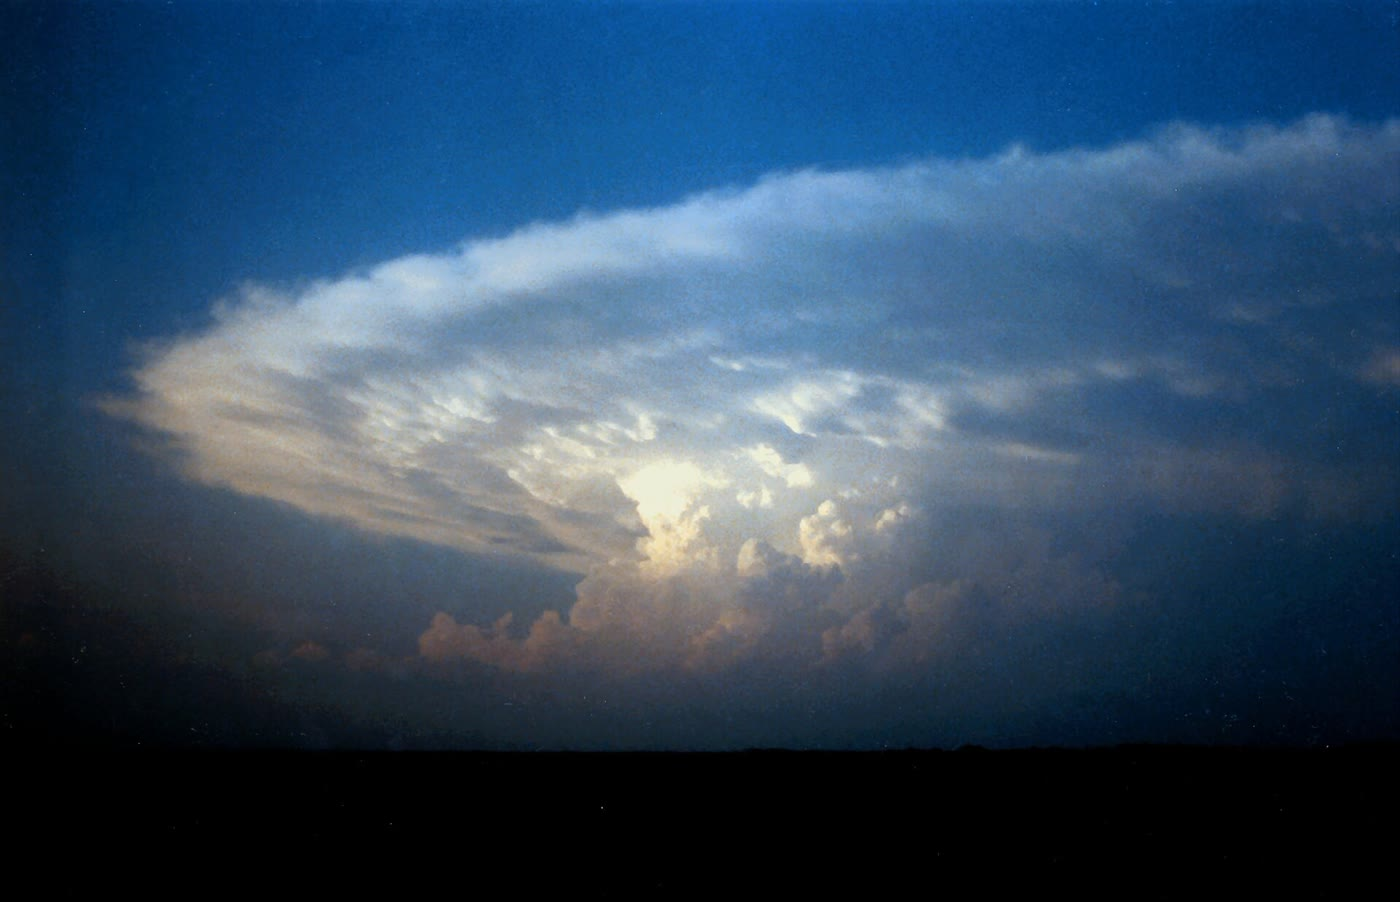
\includegraphics[width=0.6\linewidth]{images/book4/b2-21-supercell-anvil.jpg}
\par\smallskip{\small 1985 年 4 月 20 日，内布拉斯加州上空的一次雷暴：其上升气流
在接近对流层顶处铺展成砧状云，并在此抵达其\omterm{def:b2:atmospheric-thermodynamics:parcel-levels}{平衡高度}。（Stephen Corfidi，
NOAA/NWS，公有领域，经由维基共享资源提供。）}
\end{omfigure}
% ledger: nws4:lfc-el

\section{云微物理学}\label{sec:b2:atmospheric-thermodynamics:microphysics}

位于 LCL 处的气块，对平坦水面而言已饱和。液滴并不平坦：物理学教材
指出新相并非在平衡时出现，而只能经由成核形成，化学教材则说明
弯曲表面上的\omterm{def:b2:atmospheric-thermodynamics:moist-air}{水汽压}超过平坦表面上的\omterm{def:b2:atmospheric-thermodynamics:moist-air}{水汽压}，
（即开尔文方程）。依下文 \cref{prop:b2:atmospheric-thermodynamics:kohler} 中的常数 $A$，
直径为 \qty{2}{nm} 的纯水液滴，仅在饱和比
$\exp(2.1/2) = 2.9$ 时才处于平衡，\omterm{def:b2:atmospheric-thermodynamics:microphysics}{过饱和}达 \qty{190}{\percent}，远高于颗粒活化所需的百分之几：
液滴形成于颗粒之上。

\begin{definition}[过饱和；云凝结核]\label{def:b2:atmospheric-thermodynamics:microphysics}
空气的\emph{过饱和}\index{过饱和}定义为 $s = e/e_s - 1$，即其\omterm{def:b2:atmospheric-thermodynamics:moist-air}{水汽压}超出
平坦纯水面上方饱和\omterm{def:b2:atmospheric-thermodynamics:moist-air}{水汽压}的部分，通常以百分数给出。
\emph{云凝结核}\index{云凝结核}（CCN）是一种气溶胶颗粒，
在云中较小的过饱和度下，云滴即在其上形成。
它即中学分册中的\emph{凝结核}\index{凝结核}。
\end{definition}
% ledger: nws4:ccn-bergeron, pk07:kohler, morrison20:processes

\begin{proposition}[柯勒曲线]\label{prop:b2:atmospheric-thermodynamics:kohler}
\index{柯勒曲线}
直径为 $D$ 的溶液液滴生长于直径为 $D_d$ 的干颗粒上，其吸湿性为
$\kappa$，平衡时的饱和比为
\[
  S(D) = \frac{D^3 - D_d^3}{D^3 - D_d^3(1 - \kappa)}\,\exp\Bigl(\frac{A}{D}\Bigr), \qquad
  A = \frac{4\sigma M_w}{R T\rho_w},
\]
其中 $\sigma$ 为表面张力，$\rho_w$ 为水的密度（在本阶段不加证明地承认）。曲线 $S(D)$
即\emph{\omterm{prop:b2:atmospheric-thermodynamics:kohler}{柯勒曲线}}。当 $D \gg D_d$ 时，
\[
  s = S - 1 \approx \frac{A}{D} - \frac{\kappa D_d^3}{D^3},
\]
它在临界直径与临界\omterm{def:b2:atmospheric-thermodynamics:microphysics}{过饱和}度处取最大值，
\[
  D_c = \sqrt{\frac{3\kappa D_d^3}{A}}, \qquad s_c = \sqrt{\frac{4A^3}{27\,\kappa D_d^3}} .
\]
\end{proposition}
% ledger: pk07:kohler

\begin{proof}[近似的证明]
指数项即开尔文因子，分式为水的活度，是拉乌尔
定律的一种形式，其中 $\kappa$ 度量溶解物质束缚水的程度。当 $D \gg D_d$ 且
$A \ll D$ 时，$\exp(A/D) \approx 1 + A/D$，分式取一阶近似得 $1 - \kappa D_d^3/D^3$，
乘积的一阶近似为 $1 + A/D - \kappa D_d^3/D^3$。令导数
$-A/D^2 + 3\kappa D_d^3/D^4$ 为零，得 $D_c^2 = 3\kappa D_d^3/A$，于是 $s_c = A/D_c -
A/(3D_c) = 2A/(3D_c)$，即所求公式。
\end{proof}

取 $\sigma = \qty{0.072}{J/m^2}$，温度为 \qty{298.15}{K}，$A = \qty{2.1}{nm}$。硫酸铵的
$\kappa = 0.61$。氯化钠的吸湿性更强（$\kappa = 1.28$），大气颗粒多介于 0.1 与 0.9 之间。
直径 \qty{50}{nm} 的硫酸铵干颗粒，其 $D_c = \qty{0.33}{\micro m}$，$s_c =
\qty{0.42}{\percent}$；直径 \qty{100}{nm} 的颗粒则为 \qty{0.93}{\micro m} 与 \qty{0.15}{\percent}。
近似值与精确最大值相差不到 \qty{1}{\percent}。
% ledger: pk07:kohler, pk07:kappa

\begin{omfigure}
\centering
% figdata/bachelor-2/thermo.py part kohler
\begin{tikzpicture}
\begin{semilogxaxis}[width=0.72\linewidth, height=5.6cm, xmin=0.03, xmax=10, ymin=-0.4,
  ymax=1.1, xlabel={液滴直径 $D$ (\unit{\micro m})}, ylabel={过饱和度 $s$
  (\unit{\percent})}, tick label style={font=\scriptsize}, label style={font=\small},
  log ticks with fixed point, legend style={font=\scriptsize, draw=none, fill=none},
  legend pos=north east, legend cell align=left, unbounded coords=discard]
\addplot[ocBlue, thick, densely dotted] table[x=D_um, y=s30] {figdata/out/bachelor-2-thermo-kohler.dat};
\addlegendentry{$D_d = \qty{30}{nm}$}
\addplot[ocBlue, thick] table[x=D_um, y=s50] {figdata/out/bachelor-2-thermo-kohler.dat};
\addlegendentry{$D_d = \qty{50}{nm}$}
\addplot[ocBlue, thick, dashed] table[x=D_um, y=s100] {figdata/out/bachelor-2-thermo-kohler.dat};
\addlegendentry{$D_d = \qty{100}{nm}$}
\addplot[only marks, mark=*, mark size=1.5pt, black] coordinates {(0.1542,0.914) (0.3309,0.4244)
  (0.9345,0.1499)};
\draw[black!45] (axis cs:0.03,0) -- (axis cs:10,0);
\draw[ocRed, densely dashed] (axis cs:0.03,0.5) -- (axis cs:10,0.5);
\node[font=\scriptsize, ocRed, anchor=north west] at (axis cs:2.2,0.5) {$s = \qty{0.5}{\percent}$};
\end{semilogxaxis}
\end{tikzpicture}
\par\smallskip{\small 硫酸铵颗粒（$\kappa = 0.61$）三种干直径下的\omterm{prop:b2:atmospheric-thermodynamics:kohler}{柯勒曲线}，
在 \qty{298.15}{K} 下，图中圆点为其临界点。空气\omterm{def:b2:atmospheric-thermodynamics:microphysics}{过饱和}度为
\qty{0.5}{\percent} 时，\qty{50}{nm} 与 \qty{100}{nm} 的颗粒无限增长；
\qty{30}{nm} 的颗粒仍保持为霾滴。}
\end{omfigure}
% ledger: pk07:kohler, pk07:kappa

曲线将颗粒分为两类。峰值以下，液滴处于稳定平衡：若它增长，
空气的\omterm{def:b2:atmospheric-thermodynamics:microphysics}{过饱和}度已不足以维持它，它便缩回；此类霾滴
随湿度胀缩。当空气的\omterm{def:b2:atmospheric-thermodynamics:microphysics}{过饱和}度超过 $s_c$ 时，液滴
被\emph{活化}：越过峰值后，液滴增长所需的\omterm{def:b2:atmospheric-thermodynamics:microphysics}{过饱和}度越来越小，而且
只要有水汽，它便持续增长。气块上升降温，\omterm{def:b2:atmospheric-thermodynamics:microphysics}{过饱和}度随之升高，最大
且最易溶的颗粒率先活化；它们形成的液滴随之吸收水汽，
将\omterm{def:b2:atmospheric-thermodynamics:microphysics}{过饱和}度限制在一定水平。在偏远海洋上空，每立方厘米约有 110 个 CCN
在 \qty{0.4}{\percent} \omterm{def:b2:atmospheric-thermodynamics:microphysics}{过饱和}度下活化；偏远大陆上空几乎为其两倍，污染空气中约
多十倍。同样的水分散到更多液滴中，使每个液滴更小。
% ledger: andreae09:ccn, morrison20:processes

\begin{remark}[为何仅凝结不能成雨]\label{rem:b2:atmospheric-thermodynamics:growth}
液滴靠水汽向其扩散而增长。包围半径为 $r$ 的液滴的球面，
其通量为 $4\pi r D_v\,\Delta\rho_v$，其中 $D_v$ 为水汽的扩散系数，
$\Delta\rho_v$ 为远处水汽密度的过量，故其质量 $\tfrac43\pi r^3\rho_w$ 的增长
速率与 $r$ 成正比：$r\,\mathrm{d}r/\mathrm{d}t$ 为常数，$r^2$ 随时间
线性增长。大液滴比小液滴增长得慢，仅靠凝结增长的液滴群
分布变窄而非变宽。雨滴的形成，始于大小不同的液滴；
这些液滴下落速度不同，相互碰撞并合并。
\end{remark}
% ledger: morrison20:processes

在 \qty{0}{\celsius} 层以上，云由过冷液滴组成，直至冰核颗粒
开始生成冰晶。此后，饱和度图右图所示的差异
起作用：对液滴饱和的空气，相对 \qty{-10}{\celsius} 的冰面，已达 \qty{10}{\percent} \omterm{def:b2:atmospheric-thermodynamics:microphysics}{过饱和}，
这一数值为液滴活化时\omterm{def:b2:atmospheric-thermodynamics:microphysics}{过饱和}度的数十倍。
冰晶靠凝华增长，液滴因此蒸发（即贝吉龙过程，
亦即中学分册所说的冰晶过程），冰晶还会收集液滴，
使其在冰晶上冻结，此过程称凇附。
% ledger: nws4:ccn-bergeron, morrison20:processes, iapws4:sublimation

\begin{omfigure}
\centering
\begin{tikzpicture}[font=\scriptsize, box/.style={draw=black!60, rounded corners=2pt,
  align=center, minimum height=0.95cm, text width=2.1cm, fill=#1}, box/.default=white,
  >=Stealth]
\node[anchor=west, black!60] at (-1.15,0.8) {暖过程};
\node[box=black!6] (ccn) at (0,0) {气溶胶颗粒 \\(CCN)};
\node[box=ocBlue!8] (haze) at (4.2,0) {霾滴 \\$s < s_c$};
\node[box=ocBlue!15] (act) at (8.4,0) {活化液滴 \\$s > s_c$};
\node[box=ocBlue!25] (rain) at (12.6,0) {雨滴};
\draw[->] (ccn) -- node[above] {湿度} (haze);
\draw[->] (haze) -- node[above] {上升} (act);
\draw[->] (act) -- node[above, align=center] {碰撞，\\合并} (rain);
\node[anchor=west, black!60] at (-1.15,-3.4) {冰过程};
\node[box=black!6] (inp) at (0,-2.6) {冰核 \\颗粒};
\node[box=omMeth!10] (ice) at (4.2,-2.6) {冰晶 \\低于 \qty{0}{\celsius}};
\node[box=omMeth!20] (snow) at (8.4,-2.6) {雪、霰};
\node[box=ocBlue!25] (rain2) at (12.6,-2.6) {雨};
\draw[->] (inp) -- (ice);
\draw[->] (ice) -- node[above, align=center] {凝华，\\凇附} (snow);
\draw[->] (snow) -- node[above] {熔化} (rain2);
\draw[->, omMeth!60!black, dashed] (act.south) -- node[pos=0.45, right=4pt, align=left,
  omMeth!60!black] {来自蒸发液滴的 \\水汽} (ice.north);
\end{tikzpicture}
\par\smallskip{\small 水汽到降水的两条路径：液滴的活化与增长，
随后碰撞并合并（上图）；冰晶以过冷液滴为代价增长，
消耗过冷液滴并凇附，在下落进入较暖空气时熔化（下图）。}
\end{omfigure}
% ledger: morrison20:processes, nws4:ccn-bergeron

\begin{inthefield}[清晨放球]
\begin{minipage}[t]{0.54\linewidth}\vspace{0pt}
每个高空站的技术员都会在 00 和 12 UTC 前一小时内准备好气球与探空仪，
这两个时刻是全球八百多个站点同时观测的时间。
仪器重 60 至 \qty{80}{g}，悬挂于气球下方，报告气压、
气温、湿度以及卫星定位，每秒一次。气球每分钟约上升
\qty{300}{m}，持续两小时或更久，升至 \qty{35}{km} 以上方才破裂，并可能漂移
超过 \qty{300}{km}。预报员将廓线绘制在\omterm{def:b2:atmospheric-thermodynamics:diagram}{斜温对数压力图}上，并在
预计有强天气的日子，部分站点加放额外的气球。
\end{minipage}\hfill
\begin{minipage}[t]{0.42\linewidth}\vspace{0pt}
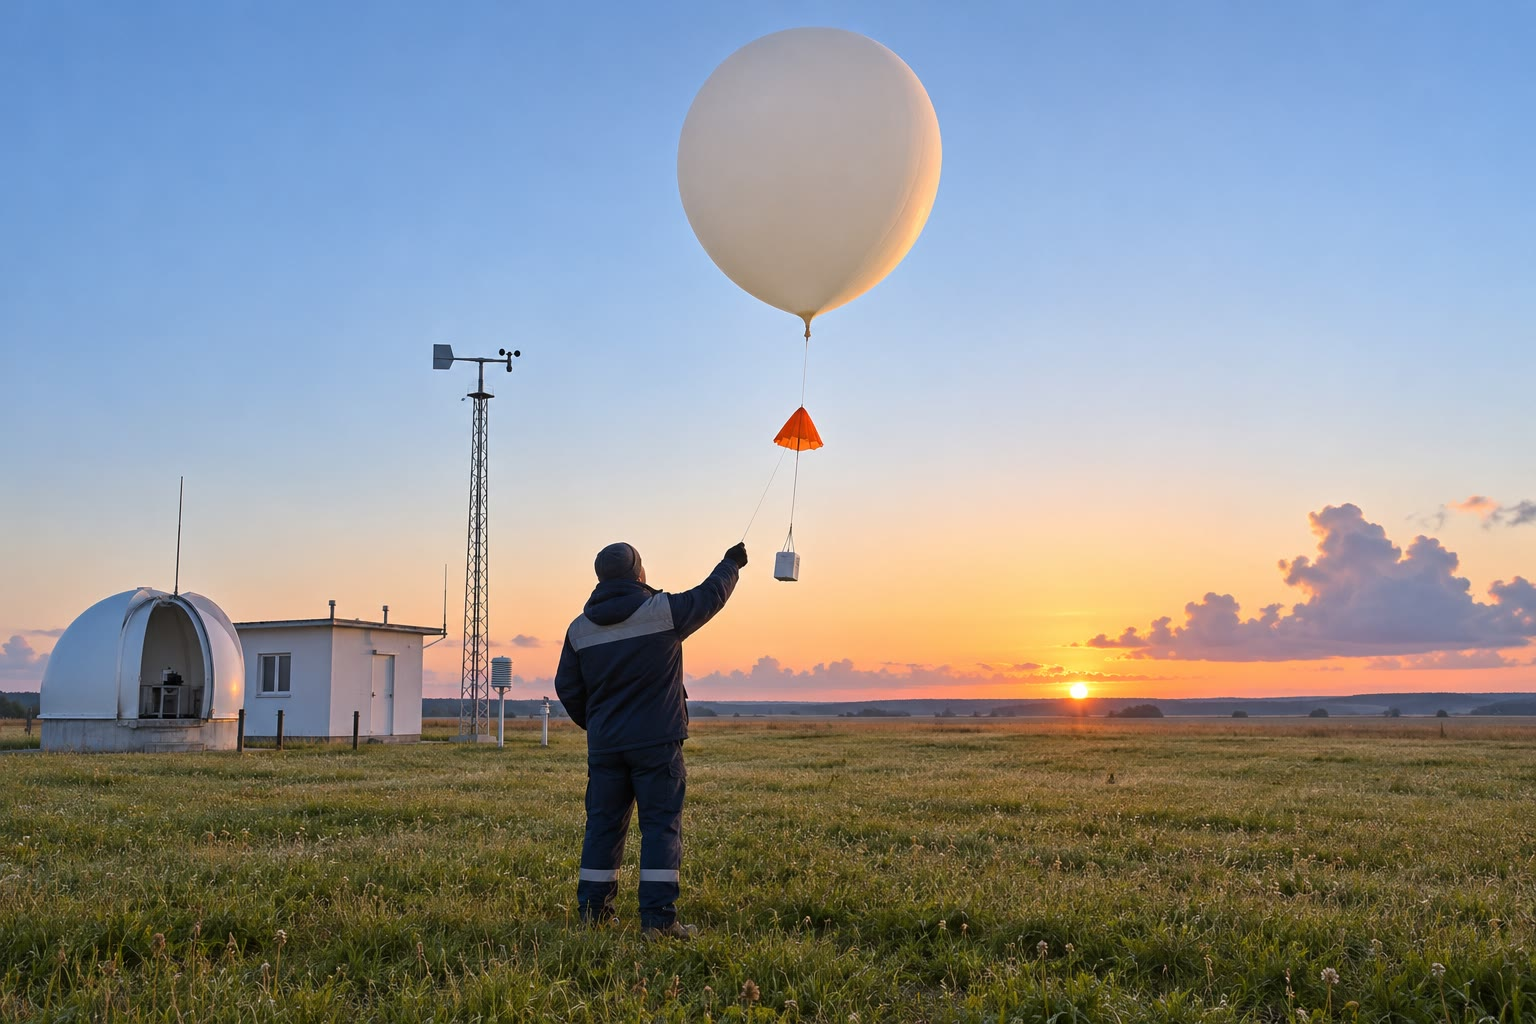
\includegraphics[width=\linewidth]{images/book4/ai/b2-radiosonde-launch.jpg}

{\scriptsize 清晨从气象站释放的探空仪（AI
生成示意图）。}
\end{minipage}
% ledger: nws:radiosonde, nws4:upperair
\end{inthefield}

\section*{练习}\label{sec:b2:atmospheric-thermodynamics:exercises}

除另有说明外，练习所用数据为：$e_s(T) = \qty{6.117}{hPa} \times
\exp[\qty{5419}{K} \times (1/\qty{273.16}{K} - 1/T)]$; $\varepsilon = 0.622$, $R_d =
\qty{287.0}{J.kg^{-1}.K^{-1}}$, $R_v = \qty{461.5}{J.kg^{-1}.K^{-1}}$, $c_p =
\qty{1004.5}{J.kg^{-1}.K^{-1}}$, $L = \qty{2.501e6}{J/kg}$, $g = \qty{9.81}{m.s^{-2}}$,
$\Gamma_d = \qty{9.8}{K/km}$.
% ledger: nist4:water-sat, iapws4:sublimation, const:R, earth:Mmol, nist4:water-mw, nasa:grc-gamma

\begin{exercise}[$\star$]\label{exo:b2:atmospheric-thermodynamics:1}
在 \qty{850}{hPa} 下，气温为 \qty{10.0}{\celsius}，露点为 \qty{5.0}{\celsius}。
(a) 求\omterm{def:b2:atmospheric-thermodynamics:moist-air}{水汽压}和饱和\omterm{def:b2:atmospheric-thermodynamics:moist-air}{水汽压}。(b) 求相对湿度。
(c) 求\omterm{def:b2:atmospheric-thermodynamics:moist-air}{混合比}和\omterm{def:b2:atmospheric-thermodynamics:moist-air}{比湿}，单位为克每千克。
\end{exercise}

\begin{exercise}[$\star$]\label{exo:b2:atmospheric-thermodynamics:2}
(a) $e_s$ 在 \qty{0}{\celsius}、\qty{20}{\celsius} 和
\qty{30}{\celsius} 时，每开尔文上升百分之几？(b) 计算 $e_s$ 在 \qty{20}{\celsius} 与 \qty{25}{\celsius} 时的值及其
比值；与 $1.063^5$ 比较。(c) 测得 \qty{20}{\celsius} 时的值为
\qty{23.39}{hPa}。公式的误差有多大？偏向哪个方向？原因何在？
\end{exercise}
% ledger: nist4:water-sat

\begin{exercise}[$\star$]\label{exo:b2:atmospheric-thermodynamics:3}
正午时地面空气温度为 \qty{30}{\celsius}，露点为 \qty{14}{\celsius}。(a) 积云云底在离地面多高处
形成？(b) 按干绝热线，气块
在该处的温度为多少？(c) 取 $\Gamma_{\text{露点}} =
\qty{1.8}{K/km}$ 时，该处的露点为多少？并加以评论。(d) 之后空气升温至 \qty{33}{\celsius}，露点
不变。此时云底在何处？
\end{exercise}

\begin{exercise}[$\star$]\label{exo:b2:atmospheric-thermodynamics:4}
读取诺曼探空的斜温图。(a) 地面附近的空气
直到哪一气压仍饱和或接近饱和？(b) 逆温层位于何处，图上如何显示？(c) 读出
地面气块的 LCL、LFC 和 EL。(d) 逆温层正上方的露点与温度
相比如何？这说明该层空气具有怎样的性质？
\end{exercise}
% ledger: data:b4-sounding

\begin{exercise}[$\star\star$]\label{exo:b2:atmospheric-thermodynamics:5}
气压为 \qty{1000}{hPa} 时，热带空气的 $T = \qty{30.0}{\celsius}$，$r = \qty{20}{g/kg}$。(a) 求
其\omterm{def:b2:atmospheric-thermodynamics:virtual}{虚温}的精确值，以及用近似式 $T(1 + 0.61\,r)$ 所得的值。(b) 求
该空气与同温同压下干空气的密度。(c) 干空气须升温多少，
才会与之同样轻？(d) 这对暖海上的对流为何重要？
\end{exercise}

\begin{exercise}[$\star\star$]\label{exo:b2:atmospheric-thermodynamics:6}
在 \qty{1000}{hPa} 下，利用 \cref{prop:b2:atmospheric-thermodynamics:gamma-s}，
并由 \cref{prop:b2:atmospheric-thermodynamics:humidity} 取 $r_s$。(a) 求 $r_s$ 与 $\Gamma_s$ 在
\qty{0}{\celsius}、\qty{20}{\celsius} 和 \qty{30}{\celsius} 时的值。(b) 饱和气块在 \qty{20}{\celsius} 时
上升 \qty{1}{km} 后，若其递减率保持不变，比干气块暖多少？
(c) 为何差值在更高处会缩小？
\end{exercise}

\begin{exercise}[$\star\star$]\label{exo:b2:atmospheric-thermodynamics:7}
诺曼地面气块（$p = \qty{971.1}{hPa}$，$T = \qty{19.0}{\celsius}$，$T_d =
\qty{18.5}{\celsius}$），其 LCL 处温度为 \qty{18.35}{\celsius}。(a) 求其\omterm{def:b2:atmospheric-thermodynamics:moist-air}{混合比}、
位温和\omterm{def:b2:atmospheric-thermodynamics:theta-e}{相当位温}。(b) 抬升至 \qty{500}{hPa} 处时，
其温度为 \qty{-8.9}{\celsius} 且已饱和，求该处的 $\theta$ 和 $\theta_e$。
(c) 两者中哪一个守恒？
\end{exercise}
% ledger: data:b4-sounding

\begin{exercise}[$\star\star$]\label{exo:b2:atmospheric-thermodynamics:8}
某气块在 \qty{700}{hPa}（其 LFC）至
\qty{300}{hPa}（其 EL）之间比周围空气暖 \qty{4}{K}，忽略\omterm{def:b2:atmospheric-thermodynamics:virtual}{虚温}修正。(a) 求其 CAPE。(b)
求 $w_{\max}$。(c) CAPE 属于哪一类？(d) 在斜温图上，正面积呈何形状，
其面积为何恰好就是所算之量？
\end{exercise}
% ledger: hgx:cape

\begin{exercise}[$\star\star$]\label{exo:b2:atmospheric-thermodynamics:9}
取 $A = \qty{2.1}{nm}$，硫酸铵的 $\kappa = 0.61$。(a) 求
\qty{80}{nm} 干颗粒的临界直径与\omterm{def:b2:atmospheric-thermodynamics:microphysics}{过饱和}度。(b) 空气在 \qty{0.3}{\percent} \omterm{def:b2:atmospheric-thermodynamics:microphysics}{过饱和}度下
能被活化的最小干颗粒为多大？在 \qty{0.1}{\percent} 时又如何？(c) 上升气流
使\omterm{def:b2:atmospheric-thermodynamics:microphysics}{过饱和}度由 \qty{0.1}{\percent} 升至 \qty{0.3}{\percent}，
液滴数目会怎样变化？相同液态水含量下，液滴尺寸又如何？
\end{exercise}
% ledger: pk07:kappa, pk07:kohler

\begin{exercise}[$\star\star\star$]\label{exo:b2:atmospheric-thermodynamics:10}
诺曼地面气块计入\omterm{def:b2:atmospheric-thermodynamics:virtual}{虚温}时，CIN 约为 \qty{-130}{J/kg}。
(a) 气块须以多大的竖直速度离开地面，
方能仅凭自身动量抵达其 LFC？(b) 逆温层顶位于 \qty{889.1}{hPa}，温度为 \qty{20.5}{\celsius}。
\qty{971.1}{hPa} 处的地面空气须升温至多少，才能使
干绝热抬升的气块不低于逆温层顶的温度？(c) 若其露点保持为 \qty{18.5}{\celsius}，
云底将在何处？(d) 说出大气不借助太阳即可
消除这类盖层的两种途径。
\end{exercise}
% ledger: data:b4-sounding, nws4:cin

\begin{exercise}[$\star\star\star$]\label{exo:b2:atmospheric-thermodynamics:11}
(a) 由 \cref{prop:b2:atmospheric-thermodynamics:gamma-s} 证明 $\Gamma_s \to \Gamma_d$，
当 $r_s \to 0$ 时成立。(b) 证明：当 $Lr_s/(R_dT) \gg 1$ 时，$\Gamma_s \to gR_vT/(LR_d)$，并
在 \qty{303}{K} 处计算该值。(c) 将其与 $\Gamma_{\text{露点}}$ 比较，
即 \cref{prop:b2:atmospheric-thermodynamics:lcl} 中 $T_d = T$ 的情形，并说明两极限为何重合。
(d) 大气中能否达到(b)中的极限？取 $\Gamma_s =
\qty{3.4}{K/km}$（\qty{30}{\celsius}，\qty{1000}{hPa}）。
\end{exercise}

\begin{exercise}[$\star\star\star$]\label{exo:b2:atmospheric-thermodynamics:12}
在过冷水面与冰面上，\qty{-10}{\celsius} 时饱和\omterm{def:b2:atmospheric-thermodynamics:moist-air}{水汽压}分别为 2.868 与
\qty{2.599}{hPa}；\qty{-20}{\celsius} 时分别为 1.257 与 \qty{1.032}{hPa}。
(a) 求水面饱和的空气在两温度下相对冰面的\omterm{def:b2:atmospheric-thermodynamics:microphysics}{过饱和}度。(b)
将其与液滴活化时的\omterm{def:b2:atmospheric-thermodynamics:microphysics}{过饱和}度相比较。(c) 解释为何
接触少量冰晶的过冷液滴云会转变为冰。(d) 为何该效应在
\qty{0}{\celsius} 附近较弱？
\end{exercise}
% ledger: iapws4:sublimation, su26:svp, nws4:ccn-bergeron

\begin{problem}[{周末问题——读取早晨探空}]\label{pb:b2:atmospheric-thermodynamics:1}
下表给出 2026 年 4 月 16 日俄克拉荷马州诺曼站 12 UTC 的探空资料，列出本文所用各层的数据：
气压、海拔高度、温度、露点，以及
按 \cref{met:b2:atmospheric-thermodynamics:lift} 所述方法抬升的地面气块温度，
由逐小步积分 \cref{prop:b2:atmospheric-thermodynamics:gamma-s} 求得。探空报告给出
对流层顶位于 \qty{235.3}{hPa}、\qty{10954}{m}。请使用习题中的数据及
温度（而非\omterm{def:b2:atmospheric-thermodynamics:virtual}{虚温}），除非另有说明。

\begin{center}
\small
\begin{tabular}{rrrrr}
\hline
$p$ (\unit{hPa}) & $z$ (\unit{m}) & $T$ (\unit{\celsius}) & $T_d$ (\unit{\celsius}) &
$T_{\text{气块}}$ (\unit{\celsius}) \\
\hline
971.1 & 345 & 19.0 & 18.5 & 19.0 \\
925.0 & 763 & 17.3 & 17.3 & 16.9 \\
907.7 & 924 & 16.4 & 16.4 & 16.2 \\
889.1 & 1102 & 20.5 & 9.5 & 15.4 \\
850.0 & 1489 & 18.6 & $-1.8$ & 13.7 \\
700.0 & 3110 & 4.5 & $-12.2$ & 6.1 \\
500.0 & 5725 & $-18.4$ & $-36.6$ & $-8.9$ \\
400.0 & 7357 & $-30.4$ & $-55.6$ & $-20.4$ \\
300.0 & 9349 & $-42.7$ & $-66.3$ & $-37.1$ \\
250.0 & 10560 & $-49.8$ & $-69.8$ & $-48.3$ \\
200.0 & 12006 & $-52.3$ & $-78.3$ & $-61.8$ \\
\hline
\end{tabular}
\end{center}

\medskip\noindent\textbf{第一部分——近地面空气。}
\begin{enumerate}
  \item 求地面空气的\omterm{def:b2:atmospheric-thermodynamics:moist-air}{水汽压}，精确到一位小数。
  \item 求其\omterm{def:b2:atmospheric-thermodynamics:moist-air}{混合比}，精确到一位小数。
  \item 求其\omterm{def:b2:atmospheric-thermodynamics:moist-air}{比湿}。
  \item 求其相对湿度。
  \item 其\omterm{def:b2:atmospheric-thermodynamics:virtual}{虚温}比温度高多少？
  \item 用 \qty{125}{m} 规则求其 LCL 离地面的高度，以及
        该处的气压（取该层平均\omterm{def:b2:atmospheric-thermodynamics:virtual}{虚温}为 \qty{294.7}{K}）。
  \item 求其位温。
\end{enumerate}

\medskip\noindent\textbf{第二部分——盖层及其上方的各层。}
\begin{enumerate}[resume]
  \item 在 \qty{925}{hPa} 处，该气块比外界更暖还是更冷？相差多少？
  \item 求 907.7 至 \qty{889.1}{hPa} 之间的递减率。这是哪一类气层？
  \item 在 \qty{889.1}{hPa} 处，该气块比外界冷多少？
  \item 求 \qty{850}{hPa} 处的相对湿度。这样的空气可能来自何处？
  \item 求 850 至 \qty{500}{hPa} 之间的平均递减率，并对该气层进行分类。
  \item 求抬升指数及其所属类别。
\end{enumerate}

\medskip\noindent\textbf{第三部分——能量。}
\begin{enumerate}[resume]
  \item 计算表中各层的超出量 $\Delta T = T_{\text{气块}} - T$。
  \item 对 $\Delta T$ 关于 $\ln p$ 作线性插值，求 LFC，精确到百帕，
        并以同样方式对 $z$ 插值，求其高度。
  \item 以同样方法求 EL 及其高度，并与对流层顶作比较。
  \item 用梯形法则在 $\ln p$ 上计算从 LFC 到 EL 的 CAPE，
        沿途经过表中各层。
  \item 它属于哪一类？
  \item 以同样方法计算 CIN，积分范围从地面到 LFC。
  \item 在 \qty{1}{hPa} 的网格上计算，用气温得 CAPE 为 \qty{2100}{J/kg}，
        用\omterm{def:b2:atmospheric-thermodynamics:virtual}{虚温}得 \qty{2230}{J/kg}，三者为何
        互不相同？
\end{enumerate}

\medskip\noindent\textbf{第四部分——空气所能驱动的风暴。}
\begin{enumerate}[resume]
  \item 取第 17 题的 CAPE，气块理论给出的竖直速度为多少？
  \item 若全程速度均为该速度的一半，空气从 LFC 上升到 EL 需要多长时间？
  \item 举出两个使实际上升气流变慢的效应。
  \item 综上所述，对于由今晨的地面空气
        所驱动的风暴，气块理论预测其上升气流速度为多少？
\end{enumerate}
\end{problem}
% ledger: data:b4-sounding, hgx:cape, nws4:lifted-index, nws4:cape
